\chapter{Geometrical Setup}\label{chap-CSXCAD}
	This chapter describes about the setup of properties and primitives of model using the \texttt{CSXCAD} interface. \texttt{CSXCAD} implies a C++ library to describe object geometries and their physical or non-physical properties in an open-source .xml format.  It provides a flexible and mesh-independent geometry definition and supports rectilinear mesh grid. CSXCAD gives absolute liberality to user in aspect of model geometry before simulating it with FDTD method using the OpenEms matlab platform. 
 
\begin{FontNameFunct}{InitCSX()}
\phantomsection \label{InitCSX}
\end{FontNameFunct}

\begin{FontDescr}{Purpose:}
In order to initiate a structure description, one should firstly choose either a Cartesian or Cylindrical coordinate based mesh definition with this function.
\end{FontDescr}

\begin{FontDescr}{Syntax:}
 \begin{lstlisting}
CSX =InitCSX();
 \end{lstlisting}
 \end{FontDescr}
 
\begin{FontDescr}{Description:}
  Initialise the \matv{CSX} data structure by defining a default cartesian mesh and return this values back to \matv{CSX}. If argument \matv{CoordSystem} with option \textcolor{green}{1} is added, the cylindrical mesh definition is set. 
  \begin{lstlisting}
CSX = InitCSX('CoordSystem','1');
  \end{lstlisting}
\end{FontDescr}
   

\section{Properties}\label{csx_prop} 
This section describes the physical and non-physical properties of a model and has to be defined before the primitive properties. 


The physical properties which can be used: 
 
\begin{enumerate}
\item Material Properties(refer to \ref{subsection_material_prop})
\item Metal (refer to \ref{subsection_metal})
\item Discretized material definition (refer to \ref{subsection_disc_material})
\item Dispersive Material(refer to \ref{subsection_dispersive_material})
\item LumpedElement(refer to \ref{subsection_lumpedelement})
\end{enumerate}


The non-physical properties which can be used: 

\begin{enumerate}
\item Electrode (refer to \ref{subsection_Electrode})
\item ProbeBox(refer to \ref{subsection_ProbeBox})
\item DumpBox (refer to \ref{subsection_DumpBox})
\end{enumerate}


\subsection{General property setup}\label{subsection_gprop_setup}
To add a physical or non-physical property into \hyperref[CSX]{\matv{CSX}}, it has a common structure as shown below:

\begin{FontDescr}{Syntax:}
\begin{lstlisting} 
CSX=Add<..property..>(CSX,name,...)
\end{lstlisting} 
\end{FontDescr}

\begin{FontDescr}{Description:}
\matv{CSX} 
\phantomsection \label{CSX}
\begin{myindentpar}
\matv{CSX} describes geometrical objects and their physical or non-physical properties in .xml file.
\end{myindentpar}

\texttt{name} 
\begin{myindentpar}
\texttt{name} is given by user and must be matched with that is mentioned in the syntax corresponding to this defined property.  
\end{myindentpar}
\end{FontDescr}


\subsection{Material Properties}\label{subsection_material_prop}

\begin{FontNameFunct}{AddMaterial()}
\end{FontNameFunct}

\begin{FontDescr}{Purpose:}
 To add specified material into \hyperref[CSX]{\matv{CSX}}.
\end{FontDescr}

\begin{FontDescr}{Syntax:}
 \begin{lstlisting}
CSX = AddMaterial(CSX, name,varargin)
 \end{lstlisting}
\end{FontDescr}

\begin{FontDescr}{Description:}
  This function adds a material property to \hyperref[CSX]{\matv{CSX}} with the given name.
\end{FontDescr}
\begin{FontDescr}{Optional Arguments:}
\begin{myindentpar} 
  \matv{Isotropy} :If it is set to be '0', an anistropy object is defined. 
\end{myindentpar}  
\end{FontDescr}

\begin{FontNameFunct}{SetMaterialProperty()}
 \end{FontNameFunct}
 
\begin{FontDescr}{Purpose:}
The material properties such as relative conductivity, permittivity and permeability can be defined with this function.
\end{FontDescr}

 \begin{FontDescr}{Syntax:}
  \begin{lstlisting}
 CSX = SetMaterialProperty(CSX, name, varargin)
  \end{lstlisting}
 \end{FontDescr}
  
 \begin{FontDescr}{Description:} 
 \begin{FontDescr}{Optional Arguments:}
  It has to be defined by user to specific the material properties.\\ 

   \textcolor{varcol}{Epsilon($\varepsilon_{r}$)}\begin{myindentpar}
     Relative permittivity [1 by default].\end{myindentpar} 

 \textcolor{varcol}{Mue($\mu_{r}$)} \begin{myindentpar}
Relative magnetic permeability[1 by default].\end{myindentpar}   

  \textcolor{varcol}{Kappa($\kappa$)} \begin{myindentpar} Electric conductivity[$\frac{S}{m}$].
\end{myindentpar} 

  \textcolor{varcol}{Sigma($\sigma$)} \begin{myindentpar}Magnetic conductivity [$\frac{\Omega}{m}$].\end{myindentpar} 

  \begin{FontPara}{Density} Material mass density[$\frac{Kg}{m^{3}}$] \end{FontPara}

   They are some frequency dependent properties which are used in describing dispersive material.Refer to \ref{subsection_dispersive_material}. 
  
 \end{FontDescr}
 \end{FontDescr}


\begin{FontNameFunct}{SetMaterialWeight}
\end{FontNameFunct}

\begin{FontDescr}{Syntax:}
  \begin{lstlisting}
 CSX = SetMaterialWeight(CSX, name, varargin)
  \end{lstlisting}
\end{FontDescr}  

\begin{FontDescr}{Purpose:}
To weight material property with known function
\end{FontDescr}

\begin{FontDescr}{Description:}
It weights a material property with given weighting function by using the variables.
\end{FontDescr}

\begin{FontDescr}{Optional Arguments:}
 The following variables can be used to define the weighting function:

\begin{FontPara}{x}{y}{z}
the distance from x,y or z along its axis to the origin
\end{FontPara}

\begin{FontPara}{rho}
the distance z-axis. It equals to $\sqrt{x^{2}+y^{2}}$
\end{FontPara}

\begin{FontPara}{r}
the distance from point to origin. It equals to $\sqrt{x^{2}+y^{2}+z^{2}}$ 
\end{FontPara}

\begin{FontPara}{a}
the polar angle as in cylindrical and spherical coordinate systems. $a=\arctan(y,x)$
\end{FontPara}

\begin{FontPara}{t}
the azimuthal angle in spherical coordinate system . $t=\arccos (z,r)$
\end{FontPara}

\end{FontDescr}


\begin{FontDescr}{Examples:}

\begin{lstlisting}
 CSX = AddMaterial( CSX, 'RO3003' );
 CSX = SetMaterialProperty( CSX, 'RO3010', 'Epsilon', 3, 'Mue', 1 );
\end{lstlisting}
 
 The first syntax adds a dielectric material named Ro3003. It has relative permittivity of 3 and relative permeability of 1. If lossy dielectric is introduced, one can set \matv{Kappa}
($\kappa$)to its correponding value with known lost tangent ($\delta$): \begin{equation}
\kappa=2*pi*freq*\varepsilon*\tan(\delta)
\end{equation} 
\begin{lstlisting}
 CSX = AddMaterial( CSX, 'RO3003' );
 CSX = SetMaterialProperty( CSX, 'RO3010', 'Epsilon', 3,'Kappa',Kappa);
\end{lstlisting}

The following example shows anisotropic material property: 

\begin{lstlisting} 
  CSX = AddMaterial( CSX, 'sheet','Isotropy',0);
  CSX = SetMaterialProperty(CSX, 'sheet', 'Kappa', [0 0 kappa]);
\end{lstlisting}

The anisotropic material named sheet has zero \matv{Kappa} at x- and y- direction but values 'kappa' at z-direction, where 'kappa' is predefined. If cylindrical coordinate system has been used, then the material sheet has only value at z-direction but not at radial and azimuthal direction. 
    
\begin{lstlisting} 
CSX = AddMaterial(CSX, 'abc');
CSX = SetMaterialProperty(CSX, 'abc', 'Epsilon', 1);
CSX = SetMaterialWeight(CSX, 'abc', 'Epsilon', ['(sin(4*z / 1000 *2*pi)>0)+1']);
\end{lstlisting}

A material named 'abc' has been added into \hyperref[CSX]{\matv{CSX}}.Its relative permittivity has been weighted with function sin depends on its z-position. 

\end{FontDescr}


\subsection{Metal}\label{subsection_metal}
 This section shows how a metal/PEC material is introduced into
 \hyperref[CSX]{\matv{CSX}}.
 
\begin{FontNameFunct}{AddMetal()}
\end{FontNameFunct}

\begin{FontDescr}{Syntax:}
  \begin{lstlisting}
 CSX = AddMetal(CSX, name)
  \end{lstlisting}
\end{FontDescr}  

\begin{FontDescr}{Description:}
This function introduces perfect electric conductor of no loss into \hyperref[CSX]{\matv{CSX}}.
\end{FontDescr}

 
\begin{FontNameFunct}{AddConductingSheet()}
\end{FontNameFunct}

\begin{FontDescr}{Purpose:}
To add a lossy conducting material into \hyperref[CSX]{\matv{CSX}}.
\end{FontDescr}

\begin{FontDescr}{Syntax:}
  \begin{lstlisting}
CSX = AddConductingSheet(CSX, name, conductivity, thickness)
  \end{lstlisting}
\end{FontDescr} 

\begin{FontDescr}{Description:}

\begin{FontPara}{conductivity}
It is given by user according to the conductivity of metal being used. The most frequent used metal is copper and its conductivity is 58e6$Sm^{-1}$.    
\end{FontPara}

 \begin{FontPara}{thickness}
 It defines the thickness of lossy metal sheet.     
 \end{FontPara}
\end{FontDescr} 

\begin{FontDescr}{Examples:} 

\begin{lstlisting} 
CSX = AddMetal(CSX,'metal'); 
\end{lstlisting}
This syntax adds PEC material into \hyperref[CSX]{\matv{CSX}} with the name 'metal'. \\

\begin{lstlisting} 
CSX = AddConductingSheet(CSX,'copper',56e6,70e-6);
\end{lstlisting}
This syntax adds a conducting sheet of 70$\mu$m into \hyperref[CSX]{\matv{CSX}}. The assigned metal is named copper and has conductivity of 58e6$Sm^{-1}$.  

 \end{FontDescr} 
 
 
 
 
 
\subsection{Discretized material definition}\label{subsection_disc_material}
 \input{chapter/SEC_CSXCAD_Setup/properties_inhomo_phantom}

\subsection{Dispersive Material}\label{subsection_dispersive_material}
 %Dispersive Material
User can model a Drude type dispersive material by function \texttt{AddLorentzMaterial()}. Dispersive material has frequency dependent relative permittivity($\varepsilon_{r}$) and permeability($\mu_{r}$), and they can be defined with function \texttt{ SetMaterialProperty()}.
\begin{equation}
\varepsilon_{r}(\omega)=\varepsilon_{r}*(1-\dfrac{\omega_{\varepsilon}^2}{\omega*(\omega-j/t_{\varepsilon})})
\end{equation}
\begin{equation}
\mu_{r}(\omega)=\mu_{r}*(1-\dfrac{\omega_{\mu}^2}{\omega*(\omega-j/t_{\mu})})
\end{equation}
where \begin{myindentpar}
\begin{itemize}
\item $\omega_{\varepsilon}$: the respective electric angular plasma frequency
\item $t_{\varepsilon}$: the electric relaxation time 
\item $\omega_{\mu}$:the respective magnetic angular plasma frequency
\item $t_{\mu}$:the magnetic relaxation time
\end{itemize}
\end{myindentpar}

\begin{FontNameFunct}{AddLorentzMaterial}
\end{FontNameFunct}

\begin{FontDescr}{Syntax:}
  \begin{lstlisting}
 CSX = AddLorentzMaterial(CSX, name)
  \end{lstlisting}
\end{FontDescr}

\begin{FontDescr}{Description:}
  This syntax adds a Drude type dispersive material model with the given name.\\ 
\end{FontDescr} 
  

\begin{FontNameFunct}{SetMaterialProperty}  
\end{FontNameFunct}\\
In this section the frequency dependent properties $\varepsilon_{r}(\omega)$ and $\mu_{r}(\omega)$ will be defined. Refer to \ref{subsection_material_prop} for non-dispersive material properties setup. 

 \begin{FontDescr}{Syntax:}
  \begin{lstlisting}
 CSX = SetMaterialProperty(CSX, name, varargin)
  \end{lstlisting}
 \end{FontDescr}
 
 \begin{FontDescr}{Arguments:}  
 
  \begin{FontPara}{EpsilonPlasmaFrequency}
  Electric plasma frequency($f_{\varepsilon}$). It equals to   $\omega_{\varepsilon}/2\pi$. 
  \end{FontPara} 
  \begin{FontPara}{MuePlasmaFrequency}($f_{\mu}$)
  Magnetic plasma frequency.It equals to $\omega_{\mu}/2\pi$.   
  \end{FontPara}
  \begin{FontPara}{EpsilonRelaxTime}   
   Electric plasma relaxation time($t_{\varepsilon}$). Smaller number results in greater losses or alternatively set it to '0' for lossless case. 
   \end{FontPara}
  \begin{FontPara}{MueRelaxTime}  
  Magnetic plasma relaxation time($t_{\mu}$).Smaller number results in greater losses or alternatively set it to '0' for lossless case.
 \end{FontPara}

For higher order Drude type, the above mentioned material constant is modified to: 

 \textcolor{varcol}{\texttt{EpsilonPlasmaFrequency$\_<n>$}}
\begin{myindentpar}
 n-th electric plasma frequency.
\end{myindentpar} 
  \textcolor{varcol}{\texttt{MuePlasmaFrequency$\_<n>$} }  
  \begin{myindentpar}
  n-th magnetic plasma frequency. 
  \end{myindentpar} 
  \textcolor{varcol}{\texttt{EpsilonRelaxTime$\_<n>$}} 
   \begin{myindentpar}
   n-th electric plasma relaxation time($t_{\varepsilon}$).   \end{myindentpar} 
 \textcolor{varcol}{\texttt{MueRelaxTime$\_<n>$}} 
\begin{myindentpar}
n-th magnetic plasma relaxation time($t_{\mu}$).
 \end{myindentpar}  
\end{FontDescr}  


\begin{FontDescr}{Example:}  
\begin{lstlisting} 
 CSX = AddLorentzMaterial(CSX,'drude');
 CSX = SetMaterialProperty(CSX,'drude','Epsilon',5,
 'EpsilonPlasmaFrequency',5e9,'EpsilonRelaxTime',1e-9);
 CSX = SetMaterialProperty(CSX,'drude','Mue',5,
 'MuePlasmaFrequency',5e9,'MueRelaxTime',1e-9);
\end{lstlisting}
  
  A Lorent material of name 'drude' has been defined. Its $\varepsilon_{r}$ and $\mu_{r}$ are set to 5 ,$f_{\varepsilon}$ and $f_{\mu}$ are both at 500M Hz while $t_{\varepsilon}$ and $t_{\mu}$ value 1e-9. 
 \end{FontDescr}
  
  
  

\subsection{LumpedElement}\label{subsection_lumpedelement}
Lumped elements like capacitor , resistor and inductor are important for tuning or matching purpose. These elements can be added into CSX with specified value and direction with function \texttt{AddLumpedElement()}. 

\begin{FontNameFunct}{AddLumpedElement}
\end{FontNameFunct}


\begin{FontDescr}{Syntax:}
  \begin{lstlisting}
CSX = AddLumpedElement(CSX, name, direction, varargin)
  \end{lstlisting}
 \end{FontDescr} 
 
\begin{FontDescr}{Description:}
\begin{FontPara}{direction}
This sets orientation of lumped elements. If a lumped element is aimed to connect two faces which are in z-direction separated, then z-orientation lumped element has to be chosen. 
 \begin{itemize}
 \item \textcolor{green}{0} :x-orientation 
 \item \textcolor{green}{1} :y-orientation
 \item \textcolor{green}{2} :z-orientation
 \end{itemize}
 \end{FontPara}
\end{FontDescr}

  
\begin{FontDescr}{Arguments:} 
 To define which lumped element to be added. 
 
 \begin{FontPara}{R}
 Lumped resistor
 \end{FontPara}
 \begin{FontPara}{C}
 Lumped capacitor
 \end{FontPara}
 \begin{FontPara}{L}
 Lumped inductor
 \end{FontPara}
 \begin{FontPara}{Caps}
It can be set to 0 or 1 to (de)activate lumped capacitor.(1=default) 
 \end{FontPara}               
 
\end{FontDescr}
 
 
\begin{FontDescr}{Example:}

\begin{lstlisting} 
CSX = AddLumpedElement( CSX, 'Capacitor', 0, 'Caps', 1, 'C', 5e-12 );
\end{lstlisting}
 A lumped capacitor in x-direction with 5pF has been added and activated. It is named as 'Capacitor'. 
\end{FontDescr}
 
non-Physical CSXProperties
\subsection{Electrode}\label{subsection_Electrode}  
Previously, the time or frequency signal excitation has been introduced in chapter~\ref{sec:FDTD_Excitation}. In this section, its geometrical distribution will be discussed. An excitation signal must be set (into \matv{FDTD}) before specifying its geometrical structure. 

Either a voltage source($U$) or a current source ($I$) can be defined with field property in function \texttt{AddExcitation()}. A voltage source can be seen as 
$\mathbf{E}$-field excitation while current source as $\mathbf{H}$-field excitation. 

    \begin{equation}
    U=\oint_{C}\vec{\mathbf{E}}.d\overrightarrow{s}
    \end{equation}
    \begin{equation}
    I=\oint_{C}\vec{\mathbf{H}}.d\overrightarrow{s}
    \end{equation}\\

\begin{FontNameFunct}{AddExcitation()}
\end{FontNameFunct}

\begin{FontDescr}{Purpose:}
Create an $\mathbf{E}$-field or $\mathbf{H}$-field excitation.
\end{FontDescr}

\begin{FontDescr}{Syntax:}
  \begin{lstlisting}
  CSX = AddExcitation(CSX, name, type, excite, varargin)
  \end{lstlisting}
\end{FontDescr}

\begin{FontDescr}{Description:}
 
A soft type field sums the from time to time updated field of the structure and field of the source while a hard type field calculate only the field of the source. It can be understood as a field locates within air enviroment for soft type field or lies near to a metal(PEC/PMC) condition for a hard type field(the total field is same as the reflected field of the source field).  

$\mathbf{E}$-field will be calculated as: 

Soft-type:
\begin{equation}
\vec{\mathbf{E}}=\vec{\mathbf{E}}_{\text{fdtd}}+\vec{\mathbf{E}}_{\text{src}} 
\end{equation}   

Hard-type:
\begin{equation}
\vec{\mathbf{E}}=\vec{\mathbf{E}}_{\text{src}}     
\end{equation}   

The same applies to $\mathbf{H}$-field.

\begin{FontPara}{type}
\textcolor{green}{0} : $\mathbf{E}$-field soft excitation \\
\textcolor{green}{1} : $\mathbf{E}$-field hard excitation\\
\textcolor{green}{2} : $\mathbf{H}$-field soft excitation\\
\textcolor{green}{3} : $\mathbf{H}$-field hard excitation\\
\textcolor{green}{10}: plane wave excitation
\end{FontPara}

\begin{FontPara}{excite}\phantomsection\label{excite_dir}
Row vector for direction of excitation.
\begin{myindentpar}
  x-or r-direction: [1 0 0] \\
  y-direction: [0 1 0] \\
  z-direction: [0 0 1] 
\end{myindentpar}
\end{FontPara}

\end{FontDescr}

\begin{FontDescr}{Additional Arguments:}

\begin{FontPara}{'Delay'} \phantomsection\label{delay}
Setup an excitation time delay in seconds. If a $x$ phase delay(in degree) at frequency $f_{1}$ is desired, 
\begin{equation}
delay= \dfrac{x}{360*f_{1}}
\end{equation}   
\end{FontPara}

\begin{FontPara}{'PropDir'} 
Only for plane wave type excitation use. Describe the direction of plane wave propagation.
\end{FontPara}
\end{FontDescr}

\begin{FontDescr}{Example:}
\begin{lstlisting} 
 CSX = AddExcitation( CSX, 'Dipole', 1, [1 0 0] );
\end{lstlisting}
An E-Field hard excitation in x-direction has been defined in \hyperref[CSX]{\matv{CSX}} with the name Dipole. 
\end{FontDescr}


\begin{FontNameFunct}{AddPlaneWaveExcite()}
\end{FontNameFunct}

\begin{FontDescr}{Purpose:}
To create a plane wave excitation in air/vacuum and
completely surround a structure. The plane wave excitation must not intersect with any kind of material. Only box property(refer to ~) can be used to describe this excitation. 

\end{FontDescr}

\begin{FontDescr}{Syntax:}
\begin{lstlisting}
CSX = AddPlaneWaveExcite(CSX, name, k_dir, E_dir, <f0, varargin>)
\end{lstlisting}
\end{FontDescr}

\begin{FontDescr}{Description:}

\textcolor{varcol}{k$\_$dir}
\begin{myindentpar}%[3em]
A row vector to describe direction of wave propagation($\vec{\mathbf{S}}$).
It must be orthorgonal to E$\_$dir. Refer to \hyperref[excite_dir]{\matv{'excite'}} in previous function for vector description.
\end{myindentpar}

\begin{equation}
\vec{\mathbf{S}}=\vec{\mathbf{E}}\times\vec{\mathbf{H}}
\end{equation}

\textcolor{varcol}{E$\_$dir} \phantomsection\label{Edir}
\begin{myindentpar}%[3em]
A row vector to describe direction of polarisation. It equals to direction of $\mathbf{E}$-field($\vec{\mathbf{E}}$). Refer to \hyperref[excite_dir]{\matv{'excite'}} in previous function for vector description. 
\end{myindentpar}
\end{FontDescr}

\begin{FontDescr}{Additional Argument:}
\begin{FontPara}{f0}
Frequency for numerical phase velocity compensation
\end{FontPara}
\end{FontDescr}

\begin{FontDescr}{Example:}
\begin{lstlisting} 
 k_dir = [1 0 0]; 
 E_dir = [0 0 1]; 
 f0 = 500e6;      
 CSX = AddPlaneWaveExcite(CSX, 'plane_wave', k_dir, E_dir, f0);
\end{lstlisting}
A plavewave excitation has been added into\hyperref[CSX]{\matv{CSX}} with the name plane$\_$wave. It is z-polarised and propagate in x-direction.  
\end{FontDescr}


\begin{FontNameFunct}{AddLumpedPort()}
\end{FontNameFunct}

\begin{FontDescr}{Purpose:}
Add a 3D geometry as excitation element.
\end{FontDescr}

\begin{FontDescr}{Syntax:}
  \begin{lstlisting}
 [CSX] = AddLumpedPort( CSX, prio, portnr, R, start, stop, dir, excitename, varargin )
  \end{lstlisting}
\end{FontDescr}

\begin{FontDescr}{Description:}
 A lumped port has been added into \hyperref[CSX]{\matv{CSX}} with the give name. 
 
\begin{FontPara}{prio}
Priority for substrate and probe boxes of the lumped port. The element of higher priority will be simulated whenever two elements of different priority are overlapping.  
\end{FontPara}

\begin{FontPara}{portnr}
Integer to represent port number. If more than one port is defined, different port numbers are recommended. 
\end{FontPara}

\begin{FontPara}{R}
Port internal resistance. For matching with the transmission line, it should be set to 50$\Omega$. 
\end{FontPara}

\begin{FontPara}{start}
A row vector to represent the starting point of the 3D geometry.
\end{FontPara}

\begin{FontPara}{stop}
A row vector to represent the end point of the 3D geometry.
\end{FontPara}

\begin{FontPara}{dir}
Direction of port. Refer to \hyperref[excite_dir]{\matv{'excite'}} in previous function.
\end{FontPara}

\begin{FontPara}{excitename}
If it is defined, the port is switched on. Else, it is only a(lossy)conducting path.
\end{FontPara}

\end{FontDescr} 

\begin{FontDescr}{Additional Argument:}
\begin{FontPara}{'Delay'}
Setup an excitation time delay in seconds. Refer to \hyperref[delay]{\matv{'delay'}} in previous function.
\end{FontPara}
\end{FontDescr} 

\begin{FontDescr}{Example:}

\begin{lstlisting} 
 start = [-0.1 -0.1 0];
 stop  = [ 0.1 0.1 5];
 [CSX] = AddLumpedPort(CSX, 5 ,1 , 50, start, stop, [0 0 1], 'excite');
\end{lstlisting}
A z-direction lumped port of dimension 0.2x0.2x5 has been switched on. It has priority of 5 and internal resistance of 50$\Omega$. If the 'excite' is omitted, this port is switched off. 
   
\begin{lstlisting} 
 start = [-0.1 -0.1 0];
 stop  = [ 0.1 0.1 5];
 [CSX] = AddLumpedPort(CSX, 5 ,1 , 50, start, stop, [0 0 1], 'excite','Delay',1/4/300e6 );
\end{lstlisting}
The port with $90^{0}$ phase shift has been switched on. 
\end{FontDescr}


\begin{FontNameFunct}{AddMSLPort()}
\end{FontNameFunct}

\begin{FontDescr}{Purpose:}
Create a MSL port with defined material property. 
\end{FontDescr}

\begin{FontDescr}{Syntax:}
  \begin{lstlisting}
[CSX,port] = AddMSLPort( CSX, prio, portnr, materialname, start, stop, dir, evec, varargin )
  \end{lstlisting}
\end{FontDescr}

\begin{FontDescr}{Description:}
\begin{FontPara}{materialname}
Property for the MSL. Function \texttt{AddMetal()}can be used to defined its property. 
\end{FontPara}

\begin{FontPara}{dir}
A number to represent wave propagation direction.\\
\textcolor{green}{0}= x-direction\\
\textcolor{green}{1}= y-direction\\
\textcolor{green}{2}= z-direction\\
\end{FontPara}

\begin{FontPara}{evec}
Refer to \hyperref[Edir]{\matv{Edir}} of function \texttt{AddLumpedPort()}. 
\end{FontPara}
\end{FontDescr}

\begin{FontDescr}{Additional Arguments:}
\begin{FontPara}{'ExcitePort'}
An excitation name.If it is defined, the port is switched on.
\end{FontPara}
\begin{FontPara}{'FeedShift'}
Shift from start to port by a given distance in drawing units. Default is 0. Only active if 'ExcitePort' is set.
\end{FontPara}
\begin{FontPara}{'MeasPlaneShift'}
Shift the measure plane to a distance specified in drawing unit. Default is the middle of start and stop vector. Only active if 'ExcitePort' is set.
\end{FontPara}

\textcolor{varcol}{'Feed$\_$R'}
Port resistance. Default is zero. It only active if 'ExcitePort' is set.

\end{FontDescr}

\begin{FontDescr}{Example:}
\begin{lstlisting} 
start=[0 0 height]; 
stop = [length width 0]; 
CSX = AddMetal( CSX, 'metal' ); %create a PEC called 'metal'
[CSX,port] = AddMSLPort( CSX, 0, 1, 'metal', start,
             stop,0, [0 0 -1],'ExcitePort','excite',     
              'Feed_R', 50 )
\end{lstlisting} 

This defines a MSL in x-direction (dir=0) with an $\mathbf{E}$-field excitation in -z-direction. The excitation is placed at x=start(1) and 
the wave travels toward x=stop(1). The MSL-metal is created in xy-plane at z=0 height by function \hyperref[addmetal]{\matv{'AddMetal()'}}.
    
\end{FontDescr}
\subsection{ProbeBox}\label{subsection_ProbeBox}  
\input{chapter/SEC_CSXCAD_Setup/probebox}
\subsection{DumpBox}\label{subsection_DumpBox}
This section introduces 'Dumpbox' property to store $\mathbf{E}$,$\mathbf{H}$-field, electrical current , current density and SAR(Specific Absorption Rate) in a specified box.  


\begin{FontNameFunct}{AddDump()}
\end{FontNameFunct}

\begin{FontDescr}{Purpose:}
Add Dumpbox property into 
\matv{CSX}\phantomsection\label{CSX} with the given name. 
\end{FontDescr}

\begin{FontDescr}{Syntax:}
\begin{lstlisting} 
 CSX = AddDump(CSX, name, varargin)
\end{lstlisting}
\end{FontDescr}

\begin{FontDescr}{Description:}

\begin{FontPara}{DumpType}
\textcolor{green}{0}: time domain $\mathbf{E}$-field \\
\textcolor{green}{1}: time domain $\mathbf{H}$-field \\
\textcolor{green}{2}: time domain electrical current($\mathbf{I}$)  \\
\textcolor{green}{3}: time domain electrical current density($\vec{\mathbf{J}}$)\\

\textcolor{green}{10}: frequency domain $\mathbf{E}$-field  \\
\textcolor{green}{11}: frequency domain $\mathbf{H}$-field\\
\textcolor{green}{12}: frequency domain electrical current($\mathbf{I}$)\\
\textcolor{green}{13}: frequency domain electrical current density($\vec{\mathbf{J}}$)\\

\textcolor{green}{20}:frequency domain local SAR \\

If this parameter is not set, the default '0' will be adopted. 
\end{FontPara}


\begin{FontPara}{DumpMode}
\textcolor{green}{0}:no-interpolation \\
\textcolor{green}{1}:node-interpolation (default DumpMode ,if it is not defined)\\
\textcolor{green}{2}:cell-interpolation

User are advised to use no- or cell-interpolation for $\mathbf{E}$-field calculation to avoid false result;use no- or node-interpolation for $\mathbf{H}$-field calculation.

\end{FontPara}

\begin{FontPara}{FileType}
  0 : vtk-file dump  (by default)\\
  1 : hdf5-file dump
\end{FontPara}

\begin{FontPara}{Frequency}
Frequency of interest for dump. 
\end{FontPara}

\end{FontDescr}

\begin{FontDescr}{Optional Arguments:}
\begin{FontPara}{SubSampling}
Field domain sub-sampling. For example, '2,2,4'. It means ?? more explanation is needed  ???
\end{FontPara}

\begin{FontPara}{OptResolution}
Field domain dump resolution, For example,'10' or '10,20,5'. It means?? more explanation is needed  ???
\end{FontPara}

\end{FontDescr}

\begin{FontDescr}{Examples:}
\begin{lstlisting} 
AddDump(CSX,'Et');
CSX = AddBox(CSX,'Et',0,[0 0 0],[100 100 200]); 
\end{lstlisting}

AddDump is added into \hyperref[CSX]{\matv{CSX}} with name Et.A box primitive with name Et has been assigned for time domain E-field(0) storage.   

\begin{lstlisting} 
AddDump(CSX,'Ef',DumpType, 10, 'Frequency',[1e9 2e9]);
CSX = AddBox(CSX,'Ef',10,[0 0 0],[100 100 200])
\end{lstlisting}

Frequency domain E-field(10)with name Ef has been 'dumped' into \hyperref[CSX]{\matv{CSX}}. The frequency of interest are 100MHz and 200MHz. These properties have been assigned to the box primitive.      

\begin{lstlisting} 
CSX=AddDump(CSX,'SAR','DumpType',20,'FileType',0,...
    'DumpMode',2,'Frequency',300e6);
CSX=AddBox(CSX,'SAR',0,[0 0 0],[100 100 200]);
\end{lstlisting}

SAR(20) at frequency 300MHz has been 'dumped' into \hyperref[CSX]{\matv{CSX}} in vtk. file type.These properties have been assigned to the box primitive.          

\end{FontDescr}


 

\section{Primitives}\label{csx_primitive} 

After defining the property of interest into 
\matv{CSX}\phantomsection\label{CSX}, user has to assign a primitive to that property by 'matching' the name of property and primitive. A warning will occur if a property without primitive has been added \matv{CSX}\phantomsection\label{CSX}. An error message will pop up if a primitive without property specification has been assigned. This primitive can be defined in either cartesian or cylindrical coordinate. The following primitives function are defined and can be added into \matv{CSX}\phantomsection\label{CSX}:   
\begin{enumerate}
\item{Point} (refer to \ref{point})
\item{Box} (refer to \ref{box})
\item{Cylinder} (refer to \ref{cylinder})
\item{CylindricalShell}(refer to \ref{cylindershell})
\item{Sphere}(refer to \ref{sphere})
\item{SphericalShell}(refer to \ref{sphereshell})
\item{Curve}(refer to \ref{curve})
\item{Wire}(refer to \ref{wire})
\item{Polygon}(refer to \ref{polygon})
\item{2D polygon}(refer to \ref{2dpoly})
\end{enumerate}

\subsection{General primitive setup} \phantomsection\label{prim_setup}
To add a primitive into \hyperref[CSX]{\matv{CSX}}, it has a common structure as shown below:

\begin{FontDescr}{Syntax:}
\begin{lstlisting} 
CSX=Add<..primitive..>(CSX,propName,prio...)
\end{lstlisting} 
\end{FontDescr}

\begin{FontDescr}{Description:}
\matv{CSX} 
\phantomsection \label{CSX}
\begin{myindentpar}
\matv{CSX} describes geometrical objects and their physical or non-physical properties in .xml file.
\end{myindentpar}

\matv{propName} 
\begin{myindentpar}
\texttt{name} is given by user and must be matched with that is mentioned in the \texttt{Add<...property...>}.Refer to \hyperref[subsection_gprop_setup]{subsection 4.1.1}.  
\end{myindentpar}

\matv{prio} 
\begin{myindentpar}
Priority of primitive.    
\end{myindentpar}
\end{FontDescr}




\subsection{Point} \phantomsection\label{point}
\input{chapter/SEC_CSXCAD_Setup/prim_point}

\subsection{Box} \phantomsection\label{box}
User can define a cube(3D),rectangular cube(3D),plane(2D),line(1D) or a point with this primitive by defining its lower-left-bottom and upper-right-top edge.

\begin{FontNameFunct}{AddBox()}
\end{FontNameFunct} 

\begin{FontDescr}{Purpose:}
Add a box to \matv{CSX}\phantomsection\label{CSX} with predefined property in either cartesian- or cylindrical- coordinate. The name of property and primitive must match.  
\end{FontDescr}

\begin{FontDescr}{Syntax:}
\begin{lstlisting} 
 CSX = AddBox(CSX, propName, prio, start, stop, varargin)
\end{lstlisting}
\end{FontDescr}

\begin{FontDescr}{Description:}

\begin{FontPara}{propName} \phantomsection \label{prim_Name}
Primitive Name which must be the same with that mentioned in the \texttt{Add<...property...>}. Refer to \hyperref[subsection_gprop_setup]{subsection 4.1.1}.
\end{FontPara}

\begin{FontPara}{start}
Start coordinate of a box.(vector)
\end{FontPara}

\begin{FontPara}{stop}
Stop coordinate of a box.(vector)
\end{FontPara}

\end{FontDescr}

\begin{FontDescr}{Optional Arguments:} \phantomsection \label{primtransform}
\begin{FontPara}{'Transform'}
Transformation of a primitive in 3D material/metal discretisation.
\begin{itemize}
\item\textcolor{varcol}{'Scale'}: scale the model with scale factor.\\ For example,'1,1,2': the z-dimension is scaled with 2. 

\item\textcolor{varcol}{'Rotate$\_$X'}:  Rotate the structure around x-axis.\\ For example, pi/4: structure will be rotated $45^{0}$. \\'Rotate$\_$Y' and 'Rotate$\_$Z' are available too.  

\item\textcolor{varcol}{'Translate'}: Translate the structure with defined distance.\\For example,'0,0,100': model will be z-direction shifted to 100 drawing unit.
\end{itemize}
\end{FontPara}
\end{FontDescr}

\begin{FontDescr}{Examples:}

\begin{lstlisting}
 CSX=InitCSX('CoordSystem',0);
 CSX = AddMetal(CSX,'metal'); 
 CSX = AddBox(CSX,'metal',10,[0 0 -100],[100 100 0]);
\end{lstlisting} 
A metal box has been defined in Cartesian coordinate and has size 100x100x100 in drawing unit.

\begin{lstlisting}
CSX=InitCSX('CoordSystem',0);
CSX = AddMetal(CSX,'metal'); 
CSX = AddBox(CSX,'metal',10,[0 0 -100],[100 100 0],
'Transform', {'Rotate_Z', pi/4});  
\end{lstlisting}  
The box is then rotated $45^{0}$ around z-axis.   

\begin{lstlisting}
 CSX=InitCSX('CoordSystem',0);
 CSX = AddMetal(CSX,'metal2'); 
 CSX = AddBox(CSX,'metal2',10,[0 0 0],[100 100 0],
 'Transform',{'Translate', '100,0,0','Scale','1/10,1,1'});
\end{lstlisting} 
This creates a strip of size 10x100 on z=0. The strip is originally created at origin with size 100x100. It is then translated to x=100 and scaled with factor 1/100 on x-dimension. The start point of strip has been transformed into x=10,y=0 and end point x=20,y=100. The translation distance has been also scaled! Refer to Fig.\ref{fig:primBoxtransform}((a),(b),(c)).

\begin{lstlisting}
 CSX=InitCSX('CoordSystem',0);
 CSX = AddMetal(CSX,'metal2'); 
 CSX = AddBox(CSX,'metal2',10,[0 0 0],[100 100 0],
 'Transform',{'Scale','1/10,1,1','Translate', '100,0,0'});
\end{lstlisting}

If scalation is done before translation, the strip will be of the same size but at different start and end point. Refer to Fig. \ref{fig:primBoxtransform}((a),(d),(e)).     

\begin{figure}[h!]
\centering
\includegraphics[width=0.85\textwidth]{svg/primBox_transform.pdf}
\caption{Transformation of strip on z-plane}
\label{fig:primBoxtransform}
\end{figure}

    
The following example will describe the box definition in cylindrical coordinate: 

\begin{lstlisting} 
 CSX=InitCSX('CoordSystem',1);
 CSX = AddMetal(CSX,'metal'); 
 CSX = AddBox(CSX,'metal',10,[-100 0 0],[100 2*pi 0]);
\end{lstlisting}
This example creates a circle of radius=100 with \texttt{AddBox} function. User can also use \texttt{AddCylinder}(section \ref{cylinder}) function to build this circle. 

\begin{lstlisting} 
 CSX=InitCSX('CoordSystem',1);
 radius=100;
 mesh_factor=[1 1/radius 1];
 CSX = AddMetal(CSX,'metal'); 
 CSX = AddBox(CSX,'metal',10,[0 0 -100].* mesh_factor,[100 100 0].* mesh_factor);
\end{lstlisting}

The metal box Fig.\ref{fig:primBoxtransform}(a) has been transformed($\Rightarrow $) into a sector of a circle with radius=100(Fig.\ref{fig:box in cyl}(a)). The dimension of a box: 

\begin{itemize}
\item x=0 $\rightarrow$ 100    $\Rightarrow $   r=0 $\rightarrow$ 100

\item y=0$\rightarrow$ 100     $\Rightarrow $   a=0 $\rightarrow$ 100/radius(=1 radian)

\item z=-100$\rightarrow$ 0   $\Rightarrow $   z=-100 $\rightarrow$ 0
\end{itemize}            

\begin{lstlisting} 
 CSX=InitCSX('CoordSystem',1);
 radius=100;
 mesh_factor=[1 1/radius 1];
 CSX = AddMetal(CSX,'metal'); 
 CSX = AddBox(CSX,'metal',10,[100 0 0].* mesh_factor,[110 100 0].* mesh_factor);
\end{lstlisting}

The strip shown in Fig.\ref{fig:primBoxtransform}(e) has been bended as it is  defined in Cylinder coordinate system(Fig.\ref{fig:box in cyl}(b)).   

\begin{itemize}
\item x=100 $\rightarrow$ 110    $\Rightarrow $   r=100 $\rightarrow$ 110

\item y=0$\rightarrow$ 100     $\Rightarrow $   a=0 $\rightarrow$ 100/radius(=1 radian)

\item z=0$\rightarrow$ 0   $\Rightarrow $   z=0 $\rightarrow$ 0
\end{itemize}  

\begin{figure}[hbt]

\centering
\subfloat[Sector of a circle]
{\includegraphics[width=0.4\textwidth]{svg/box_cylinderco.pdf}}
\subfloat[Bended strip]{\includegraphics[width=0.41\textwidth]{svg/bended_strip.pdf}}
\caption{Top view of the transformed box(a) and strip(b).}
\label{fig:box in cyl}
\end{figure}

\end{FontDescr}




\subsection{Cylinder } \phantomsection\label{cylinder}
Introduce a cylinder into\hyperref[CSX]{\matv{CSX}} with predefined matlab function \texttt{AddCylinder}.

\begin{FontNameFunct}{AddCylinder()}
\end{FontNameFunct}

\begin{FontDescr}{Purpose:}
Define cylinder with its axis(where it extends) and radius and assign a property to it. 
\end{FontDescr}

\begin{FontDescr}{Syntax:}
\begin{lstlisting} 
 CSX = AddCylinder(CSX, propName, prio, start, stop, rad, varargin)
\end{lstlisting}
\end{FontDescr}

\begin{FontDescr}{Description:}

\begin{FontPara}{propName}
Refer to \hyperref[prim_Name]{propName} in \texttt{AddBox}. 
\end{FontPara}

\begin{FontPara}{start}
A vector represents start point of cylinder axis.  
\end{FontPara}

\begin{FontPara}{stop}
End point of cylinder axis(vector). Extend in the same direction as start point.  
\end{FontPara}

\begin{FontPara}{rad}
Radius of cylinder. In drawing unit. 
\end{FontPara}
\end{FontDescr}

\begin{FontDescr}{Optional Arguments:}
The standard trasformation (rotation,translation,scaling) mentioned in  \hyperref[prim_transform]{\matv{'Transform'}} of \texttt{AddBox}.  
\end{FontDescr}

\begin{FontDescr}{Examples:}

\begin{lstlisting} 
CSX=AddMaterial(CSX,'phantom');
CSX=SetMaterialProperty(CSX,'phantom','Epsilon',75.5,
'Kappa',0.438,'Density',1000);
start=[0 0 -30 ];
stop=[0 0 30 ];
CSX=AddCylinder(CSX,'phantom',5,start,stop,10);
\end{lstlisting}
This example introduces a 10(drawing unit) radius homogeneous phantom into\hyperref[CSX]{\matv{CSX}}. This phantom has properties of $\varepsilon_{r}$=75.5, $\kappa$=0.438 and density of 1000. It extends in z-direction and has 60(drawing unit)height.  

\end{FontDescr}


\subsection{CylindricalShell} \phantomsection\label{cylindershell}
Introduce a cylindrical shell into\hyperref[CSX]{\matv{CSX}}. 

\begin{FontNameFunct}{AddCylindricalShell()}
\end{FontNameFunct}


\begin{FontDescr}{Purpose:}
To add cylinder with specified shell width to\hyperref[CSX]{\matv{CSX}}. 
\end{FontDescr}

\begin{FontDescr}{Syntax:}
\begin{lstlisting} 
 CSX = AddCylindricalShell(CSX, propName, prio, start, stop, rad, shell_width, varargin)
\end{lstlisting}
\end{FontDescr}

\begin{FontDescr}{Description:}
The parameters are defined same as those in \texttt{Addcylinder}(\ref{cylinder}) except the following: \\
\textcolor{varcol}{shell$\_$width}
\begin{myindentpar} Width of the shell. The inner radius($r_{in}$) and outer radius($r_{out}$) of shell are:

\begin{equation}    
r_{in}=rad-shell_width/2 
\end{equation}
\label{rin}
\begin{equation}
r_{out}=rad+shell_width/2 
\end{equation}
\label{rout}

\end{myindentpar} 

\end{FontDescr}

\begin{FontDescr}{Optional Arguments:}
The standard trasformation (rotation,translation,scaling) mentioned in  \hyperref[prim_transform]{\matv{'Transform'}} of \texttt{AddBox}.   
\end{FontDescr}

\begin{FontDescr}{Examples:}

\begin{lstlisting} 
CSX=AddMaterial(CSX,'plexi_shield');
CSX=SetMaterialProperty(CSX,'plexi_shield','Epsilon'
,2.22);
start=[0 0 -30 ];
stop=[0 0 30 ];
CSX=AddCylindricalShell(CSX,'plexi_shield',5,start,stop,
20,10);
\end{lstlisting}
A cylinder shell of radius 20 and shell width of 10 has defined around z-axis.It has dielectric material property($\varepsilon_{r}$=2.22) and height of 60. The inner radius of cylindrical shell is 20-10/2=15 ; the outer radius of it is 20+10/2=25 drawing unit.    
\end{FontDescr}



\subsection{Sphere} \phantomsection\label{sphere}
Introduce a sphere into\hyperref[CSX]{\matv{CSX}}. 

\begin{FontNameFunct}{AddSphere()}
\end{FontNameFunct}


\begin{FontDescr}{Purpose:}
To add a sphere into\matv{CSX}\phantomsection\label{CSX} by defining its radius and center point and assign a material property to it.  
\end{FontDescr}

\begin{FontDescr}{Syntax:}
\begin{lstlisting} 
CSX = AddSphere(CSX, propName, prio, center, rad, varargin)
\end{lstlisting}
\end{FontDescr}

\begin{FontDescr}{Description:}

\begin{FontPara}{propName}
Refer to \hyperref[prim_Name]{propName} in \texttt{AddBox}. 
\end{FontPara}

\begin{FontPara}{center}
Sphere center point.(Vector) 
\end{FontPara}

\begin{FontPara}{rad}
Radius of a sphere.
\end{FontPara}
\end{FontDescr}

\begin{FontDescr}{Optional Arguments:}
The standard trasformation (rotation,translation,scaling) mentioned in  \hyperref[prim_transform]{\matv{'Transform'}} of \texttt{AddBox}.   
\end{FontDescr}

\begin{FontDescr}{Examples:}

\begin{lstlisting} 
CSX = AddMetal(CSX,'metal'); 
CSX = AddSphere(CSX,'metal',10,[0 0 0],50);
\end{lstlisting}
This example creates a metallic sphere of radius 50(drawing unit) at origin. 

\begin{lstlisting} 
CSX = AddMetal(CSX,'metal'); 
CSX = AddSphere(CSX,'metal1',10,[0 0 0],10,'Transform',{'Translate','0,0,50'});  
\end{lstlisting}
The above sphere has been shifted in z-direction 50(drawing unit) above the origin. 

\end{FontDescr}





\subsection{SphericalShell} \phantomsection\label{sphereshell}
Introduce a spherical shell into\hyperref[CSX]{\matv{CSX}}. 

\begin{FontNameFunct}{AddSphericalShell()}
\end{FontNameFunct}

\begin{FontDescr}{Purpose:}
To add a spherical shell in\hyperref[CSX]{\matv{CSX}} by defining its radius, center point and shell width. 
\end{FontDescr}

\begin{FontDescr}{Syntax:}
\begin{lstlisting}
CSX = AddSphericalShell(CSX, propName, prio, center, rad, shell_width, varargin) 
\end{lstlisting}
\end{FontDescr}

\begin{FontDescr}{Description:}
The parameters are defined same as those in \texttt{AddSphere}(subsection~\ref{sphere}) except the following: \\
\textcolor{varcol}{shell$\_$width}
\begin{myindentpar} Width of the shell. The inner radius and outer radius of shell is calculated as shown in \hyperref[rin]{$r_{in}$} and \hyperref[rout]{$r_{out}$} of section \ref{cylindershell}.
\end{myindentpar} 
\end{FontDescr}

\begin{FontDescr}{Optional Arguments:}
The standard trasformation (rotation,translation,scaling) mentioned in  \hyperref[prim_transform]{\matv{'Transform'}} of \texttt{AddBox}.   
\end{FontDescr}

\begin{FontDescr}{Examples:}

\begin{lstlisting} 
 CSX = AddMetal(CSX,'metal'); 
 CSX = AddSphericalShell(CSX,'metal',10,[0 0 0],50,10);
\end{lstlisting}
A metallic spherical shell of radius 50 has been added into\hyperref[CSX]{\matv{CSX}}. The thickness of shell is 10. So, the inner radius of shell is 50-10/2=45 while outer radius of shell is 50+10/2=55.   

\begin{lstlisting} 
 CSX = AddMetal(CSX,'metal'); 
 CSX = AddSphericalShell(CSX,'metal',10,[0 0 0],50,10,'Transform',{'Scale','3,3,3'});
\end{lstlisting}
The above mentioned spherical shell has been scaled with factor 3. It is 3 times larger than original size. 

\end{FontDescr}

\subsection{Curve} \phantomsection\label{curve}
Introduce a curve into \hyperref[CSX]{\matv{CSX}} with matlab function \texttt{AddCurve} and assign a property to it. 

\begin{FontNameFunct}{AddCurve()}
\end{FontNameFunct}


\begin{FontDescr}{Purpose:}
Add 1D curve to \hyperref[CSX]{\matv{CSX}} by defining its coordinate arrays.
\end{FontDescr}

\begin{FontDescr}{Syntax:}
\begin{lstlisting} 
 CSX = AddCurve(CSX, propName, prio, points, varargin)
\end{lstlisting}
\end{FontDescr}

\begin{FontDescr}{Description:}

\begin{FontPara}{propName}
Refer to \hyperref[prim_Name]{propName} in \texttt{AddBox}. 
\end{FontPara}

\begin{FontPara}{points}
\phantomsection \label{points_curve}
Curve coordinates array. Array column refers to point number while array row refers to its x,y,z- position:
\begin{myindentpar}     
points(1,point$\_$number): position-x of point.\\
points(2,point$\_$number): position-y of point.\\
points(3,point$\_$number): position-z of point.
\end{myindentpar}

\end{FontPara}
\end{FontDescr}

\begin{FontDescr}{Optional Arguments:}
The standard trasformation (rotation,translation,scaling) mentioned in  \hyperref[prim_transform]{\matv{'Transform'}} of \texttt{AddBox}.   
\end{FontDescr}


\begin{FontDescr}{Examples:}

\begin{lstlisting} 
%first point
     points(1,1) = 0;points(2,1) = 5;points(3,1) = 10; 
%second point
     points(1,2) = 0;points(2,2) = 10;points(3,2) = 10; 
     CSX = AddMetal(CSX,'metal'); 
     CSX = AddCurve(CSX,'metal',10, points);
\end{lstlisting}
This example creates a thin metallic wire from y=5 to y=10(5 drawing unit long).

\begin{lstlisting} 
    points(1,1) =  0;points(2,1) = 0;points(3,1) = 0;
    points(1,2) =  5;points(2,2) = 0;points(3,2) = 5;
    points(1,3) = 10;points(2,3) = 0;points(3,3) = 0.5;
    points(1,4) = 15;points(2,4) = 0;points(3,4) = 5;
    points(1,5) = 20;points(2,5) = 0;points(3,5) = 0;
    points(1,6) = 15;points(2,6) = 0;points(3,6) = -5;
    points(1,7) = 10;points(2,7) = 0;points(3,7) = -0.1;
    points(1,8) =  5;points(2,8) = 0;points(3,8) = -5;
    points(1,9) =  0;points(2,9) = 0;points(3,9) = 0;
    CSX = AddMetal(CSX,'metal'); 
    CSX = AddCurve(CSX,'metal',10, points);
\end{lstlisting}
This example creates a Biquad antenna from thin wire on y=0, with length of each side=$\sqrt{50}$.
\end{FontDescr}

\begin{figure}[hbt]
\centering
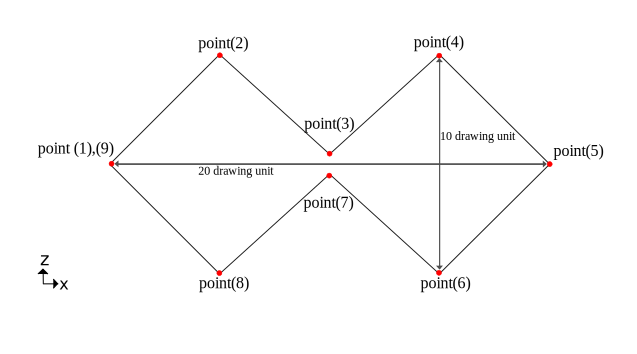
\includegraphics[width=0.8\textwidth]{svg/biquad_prim_curve.pdf}
\caption{Biquad antenna with side length $\sqrt{50}$ in xz-plane.}
\label{fig:primCurve}
\end{figure}

\subsection{Wire} \phantomsection\label{wire}
Introduce a curve with defined radius into \hyperref[CSX]{\matv{CSX}} with matlab function \texttt{AddWire} and assign a property to it. 

\begin{FontNameFunct}{AddWire()}
\end{FontNameFunct}


\begin{FontDescr}{Purpose:}
Add wire to \hyperref[CSX]{\matv{CSX}} by defining its coordinate arrays and radius. Take note that wire is not a solid cylinder!  
\end{FontDescr}

\begin{FontDescr}{Syntax:}
\begin{lstlisting} 
 CSX = AddWire(CSX, propName, prio, points, wire_rad, varargin)
\end{lstlisting}
\end{FontDescr}

\begin{FontDescr}{Description:}

\begin{FontPara}{propName}
Refer to \hyperref[prim_Name]{propName} in \texttt{AddBox}. 
\end{FontPara}

\begin{FontPara}{points}
Refer to parameter \hyperref[points_curve]{\matv{points}} in section \ref{curve}.
\end{FontPara}

\textcolor{varcol}{wire$\_$rad}
\begin{myindentpar}
Wire radius. 
\end{myindentpar}
\end{FontDescr}

\begin{FontDescr}{Optional Arguments:}
The standard trasformation (rotation,translation,scaling) mentioned in  \hyperref[prim_transform]{\matv{'Transform'}} of \texttt{AddBox}.   
\end{FontDescr}

\begin{FontDescr}{Examples:}
\begin{lstlisting} 
%first point
     points(1,1) = 0;points(2,1) = 5;points(3,1) = 0; 
%second point
     points(1,2) = 0;points(2,2) = 5;points(3,2) = 100; 
     CSX = AddMetal(CSX,'metal'); 
     CSX = AddWire(CSX,'metal',10, points,2);
\end{lstlisting}
This example creates a metallic 100 unit long wire.This wire is hollow cylinder with defined radius and very thin shell width.   
\end{FontDescr}


\subsection{Polygon} \phantomsection\label{polygon}
\input{chapter/SEC_CSXCAD_Setup/prim_poly}

\subsection{2D polygon} \phantomsection\label{2dpoly}
\input{chapter/SEC_CSXCAD_Setup/prim_2dpoly}

 \label{CSXprimitives} 

